\chapter{Situationsanalyse}

\section[Software-Qualität]{Software-Qualität~\footcite[vgl.][Kapitel 1.2]{hoffmann_software-qualitat_2013}}

Eine mögliche Definition von Software-Qualität findet sich in der DIN-ISO-Norm 9126:

\begin{quote}
  Software-Qualität ist die Gesamtheit der Merkmale und Merkmalswerte eines Software-Produkts, die sich auf dessen Eignung beziehen, festgelegte Erfordernisse zu erfüllen.
\end{quote}

Wie aus dieser Definition schon erkennbar ist, gibt es viele unterschiedliche Kriterien, um die Qualität von Software zu bewerten.
Einige wesentliche Merkmale, um die Qualität von Software bewerten zu können, lassen sich in kunden- und herstellerorientierte Merkmale unterteilen:

\begin{description}
  \item[Kundenorientierte Merkmale] \hfill \\ Nach außen hin sichtbare Merkmale, die sich auf den kurzfristigen Erfolg der Software auswirken, da sie die Kaufentscheidung möglicher Kunden beeinflussen.
  \begin{description}
    \item[Funktionalität (Functionality, Capability)] \hfill \\ Beschreibt die Umsetzung der funktionalen Anforderungen. Fehler sind hier häufig Implementierungsfehler (sogenannte Bugs), welche durch Qualitätssicherung bereits in der Entwicklung entdeckt oder vermieden werden können. 
    \item[Laufzeit (Performance)] \hfill \\ Beschreibt die Umsetzung der Laufzeitanforderungen. Besonderes Augenmerk muss in Echtzeitsystemen auf dieses Merkmal gelegt werden.
    \item[Zuverlässigkeit (Reliability)] \hfill \\ Eine hohe Zuverlässigkeit ist in kritischen Bereichen, wie z.B. Medizintechnik oder Luftfahrt, unabdingbar. Erreicht werden kann diese aber nur durch die Optimierung einer Reihe anderer Kriterien.
    \item[Benutzbarkeit (Usability)] \hfill \\ Betrifft alle Eigenschaften eines Systems, die mit der Benutzer-Interkation in Berührung kommen.
  \end{description}
  \item[Herstellerorientierte Merkmale] \hfill \\ Sinf die inneren Merkmale, die sich auf den langfristigen Erfolg der Software auswirken und somit als Investition in die Zukunft gesehen werden sollten.
  \begin{description}
    \item[Wartbarkeit (Maintainability)] \hfill \\ Die Fähigkeit auch nach der Inbetriebnahme noch Änderungen an der Software vorzunehmen. Wird oft vernachlässigt, ist aber essentiell für langlebige Software und ein großer Vorteil gegenüber der Konkurrenz.
    \item[Transparenz (Transparency)] \hfill \\ Beschreibt, wie die nach außen hin sichtbare Funktionalität intern umgesetzt wurde. Gerade bei alternder Software, kann es zu einer Unordung kommen, welche auch Software-Entropie (Grad der Unordnung) genannt wird.
    \item[Übertragbarkeit] \hfill \\ Wird auch Portierbarkeit genannt und beschreibt die Eigenschaft einer Software, in andere Umgeungen übertragen werden zu können (z.B. 32-Bit zu 64-Bit oder Desktop zu Mobile).
    \item[Testbarkeit (Testability)] \hfill \\ Testen stellt eine große Herausforderung dar, da oft auf interne Zustände zugegriffen werden muss oder die Komplexität die möglichen Eingangskombinationen vervielfacht. Aber gerade durch Tests können Fehler frühzeitig entdeckt und behoben werden.
  \end{description}
\end{description}

Je nach Anwendungsgebiet und den Anforderungen der Software haben die Merkmale unterschiedliche Relevanz und einige können sich auch gegenseitig beeinflussen, wie aus der Korrelationsmatrix ersichtlich.

\begin{savenotes}
  \begin{figure}[H] 
    \centering
       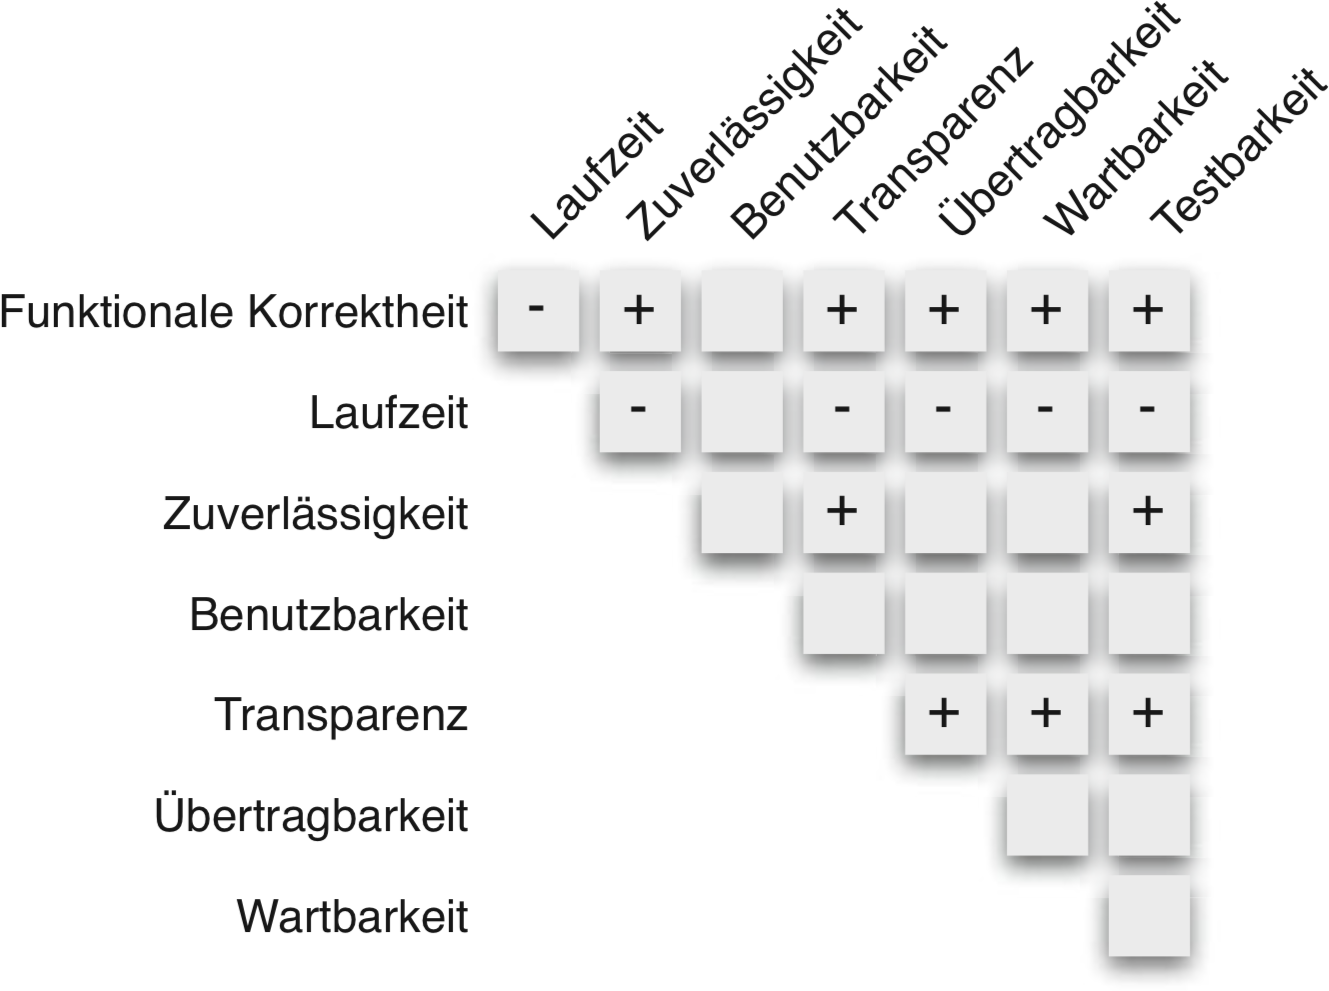
\includegraphics[width=0.6\textwidth]{img/korrelationsmatrix-kriterien.png}
    \caption[Korrelationsmatrix Qualitätskriterien]{Korrelationsmatrix Qualitätskriterien~\footcite[][S. 11, Abb. 1.3]{hoffmann_software-qualitat_2013}}
    \label{fig:Korrelationsmatrix Qualitätskriterien}
  \end{figure}
\end{savenotes}
